% !TeX spellcheck = en_US
\section{Race Detection by Mining Locking Rules}
\label{sec_technique}
To address the above challenges, we propose three key techniques. For {\em C1}, 
we propose an {\em alias-aware rule mining method} to automatically deduce 
locking rules. For {\em C2}, we propose a {\em lock-usage analysis} to filter 
out false data races by validating concurrency of code paths. For {\em C3}, we 
propose a pattern-based estimation to extract harmful races that can trigger 
memory or logical bugs such as null-pointer dereference and data inconsistency. 
We introduce them as follows:

\subsection{Alias-Aware Rule Mining Method}
\label{subsec_rule_mining}
The relationship between variables and locks are not well documented in OS 
kernels, but it can be inferred from the kernel code. Specifically, a variable 
is often protected by the lock stored in the same data structure. And thus if a 
variable is accessed after acquiring a lock existing in the same data structure 
in most cases, it is likely to be protected by the lock. Whether a variable and 
the protecting lock exist in the same data structure can be determined though 
an alias graph~\cite{Li:ASPLOS22, Kastrinis:CC18} by finding their common 
ancestor. Based on this insight, we propose an {\em alias-aware rule mining 
method} to deduce locking rules automatically. Moreover, with benefits from 
precise field-sensitive alias relationships of alias graph, our alias-aware 
rule mining method can find data structure filed and its protecting lock 
effectively.

\PP{Alias Graph.} It is an important data structure to infer relationships 
between variable and its protecting lock in our analysis, so we introduce it 
and its update first. 

An alias graph is a 2-tuple $\mathit{G = \left<N, E\right>}$, where 
$\mathit{N}$ is a set of nodes, and each node $\mathit{n}$ represents an alias 
set that points to one abstract object. $\mathit{E}$ is a set of labeled edges. 
Each edge is labeled with a data structure field or a dereference operator 
``$\mathit{*}$'', which represents how an abstract object is accessed. In an 
alias node, a variable residing in a node followed by a sequence of edge
labels form an access path~\cite{Kastrinis:CC18, Cheng:PLDI00}. In this paper, 
we replace the variable in an access path with its structure name to represent 
a data structure field.

An alias graph is updated by handling four types of instructions that  
change alias relationships: MOVE($\mathit{v_1 = v_2}$), STORE ($\mathit{*v_2 = 
v_1}$), LOAD ($\mathit{v_1 = *v_2}$) and GEP ({$\mathit{v_1 = \&v_1->f}$}). We 
exploit {$\mathit{n_x}$} to represent the node whose representing alias set 
includes $\mathit{v_x}$, and introduce how the four types of instructions 
update alias graphs. For a MOVE operation, $\mathit{v_1}$ is moved from 
$\mathit{n_1}$ to $\mathit{n_2}$. After this operation, $\mathit{v_1}$ and  
$\mathit{v_2}$ are represented by the same node, which indicates they become 
aliases. For a STORE operation, the existing outgoing edge from $\mathit{n_2}$ 
is dropped first, and then a new edge labeled with $\mathit{*}$ from 
$\mathit{n_2}$ to $\mathit{n_1}$ is inserted. After this operation, 
$\mathit{v_1}$ and $\mathit{*v_2}$ are represented by the same node, which 
indicates they become aliases. For a LOAD operation, the analysis first finds 
the destination node of the edge that comes from $\mathit{n_2}$ and is labeled 
with $\mathit{*}$, and then move $\mathit{v_1}$ to the destination node. And 
after this operation, $\mathit{v_1}$ and $\mathit{*v_2}$ are represented by the 
same node, which indicates they become aliases. GEP operation is similar to 
LOAD, expect that the edge is labeled with a data structure field $\mathit{f}$, 
instead of a dereference operator $\mathit{*}$.

\begin{figure}[htbp]
	\centering
	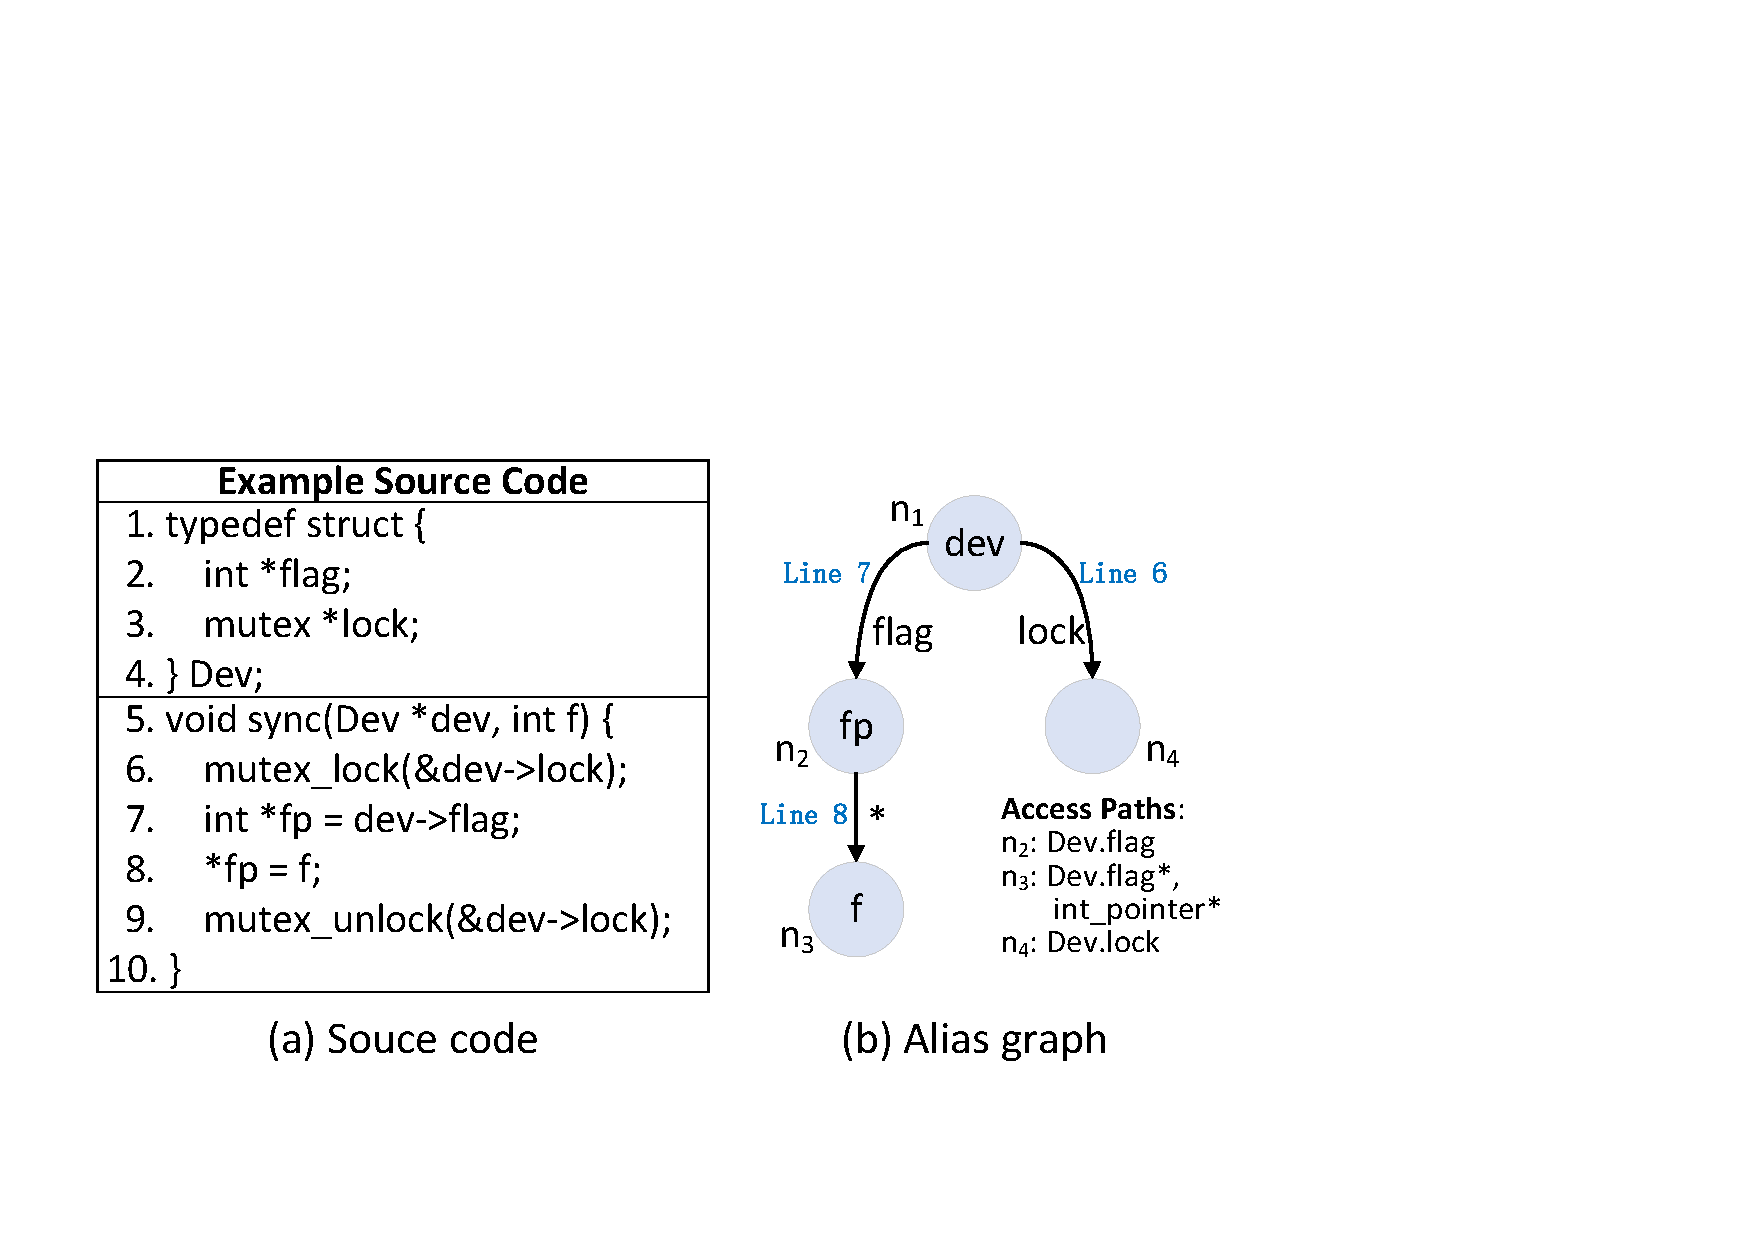
\includegraphics[width=0.9\linewidth]{figures/fig_demo_alias_graph.pdf}
	\figcaption{Example of alias graph.}
	\label{fig_demo_alias_graph}
\end{figure}

\noindent{\textbf{\em Example.}} Figure~\ref{fig_demo_alias_graph} shows a 
piece of driver-like source code and its alias graph. In this example, after an 
GEP (\&dev->lock) operation at Line 6, an edge labeled with {\tt lock} from 
node $\mathit{n_1}$ to node $\mathit{n_4}$ is inserted. Similarly, an edge 
labeled with {\tt flag} from node $\mathit{n_1}$ to node $\mathit{n_2}$ is 
inserted after Line 7. At last, an edge labeled with a dereference operator 
($\mathit{*}$) is inserted after the STORE (*fp = f) operation at Line 8. The 
final alias graph is shown in Figure~\ref{fig_demo_alias_graph}(b), and access 
paths are shown in the bottom left corner. Take node $\mathit{n_3}$ as an 
example, it can represent two fields, one is {\tt Dev.flag*}, and the other is 
{\tt int\_pointer*} (we exploit int\_pointer to represent a pointer points to 
an integer, and regard it as a data structure for convenience). 

\begin{figure}[htbp]
	\centering
	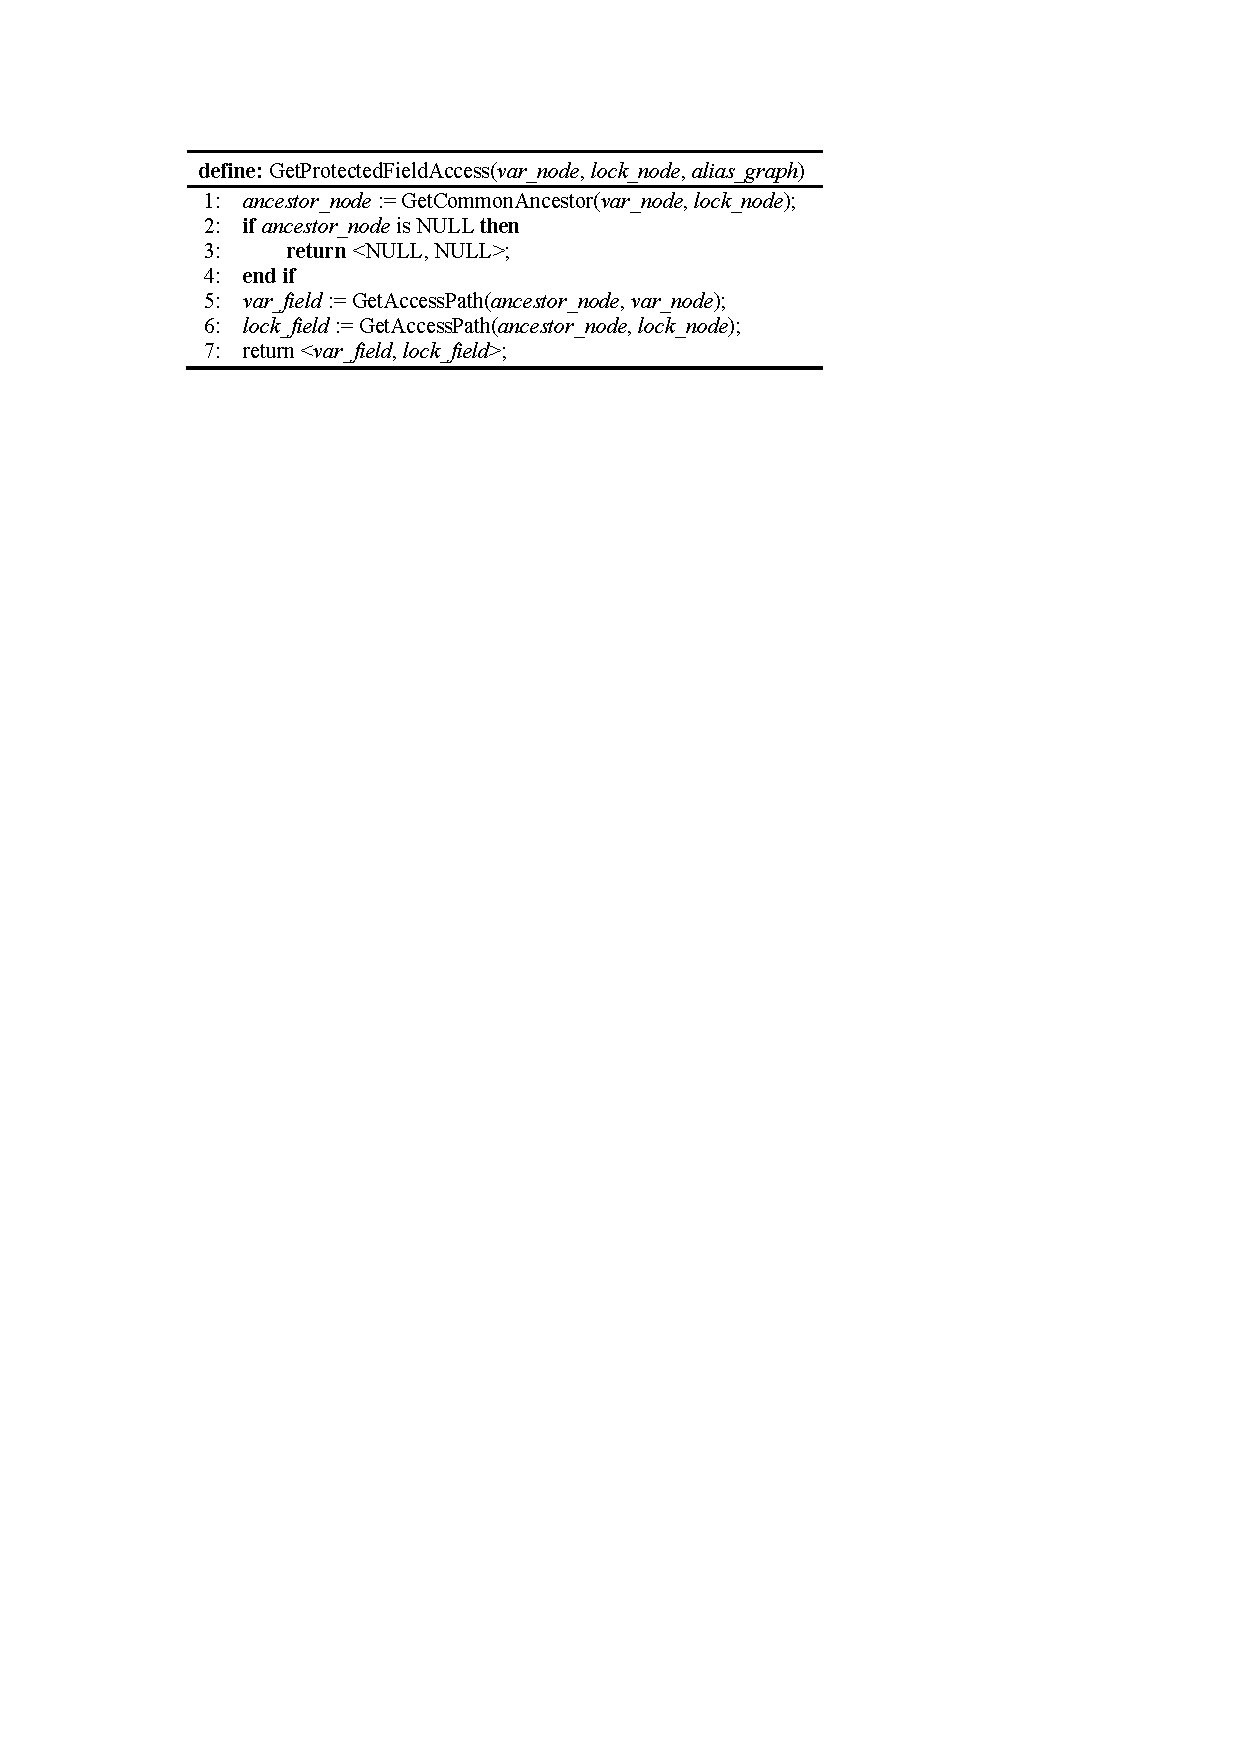
\includegraphics[width=1\linewidth]{figures/fig_pseudocode_get_access.pdf}
	\figcaption{Pseudocodes to get accessed field and protecting lock.}
	\label{fig_pseudocode_get_access}
\end{figure}

Given an alias graph, whether a variable and a lock exist in the same data 
structure can be determined by finding a common ancestor. If they are in the 
same data structure, the lock is likely to protect the variable when it is 
accessed. Figure~\ref{fig_pseudocode_get_access} shows the pseudocode to 
get the field of the accessed variable and the field of the protecting lock in 
the form of access path, if they exist in the same data structure. Given a node 
of an accessed variable and a node of a lock variable, the analysis first gets 
the common ancestor of the two nodes (Line 1). And then, if the common ancestor 
does not exist, the analysis returns a NULL pair (Lines 2-3). Otherwise, the 
analysis gets the access path for the node of the accessed variable and the 
node of the lock variable from the common ancestor (Lines 5-7).

Take the alias graph in Figure~\ref{fig_demo_alias_graph} as an example, {\tt 
\&dev->flag} is represented by node $\mathit{n_2}$, and {\tt \&dev->lock} is 
represented by node $\mathit{n_4}$. The two nodes have a common ancestor 
$\mathit{n_1}$, and thus the accessed variable {\tt \&dev->flag} and the 
protecting lock {\tt \&dev->lock} can be inferred to exist in the same data 
structure (namely {\tt Dev}). Therefore, the structure field Dev.flag is likely 
to be protected the lock stored in the structure field Dev.lock.

\begin{figure}[htbp]
	\centering
	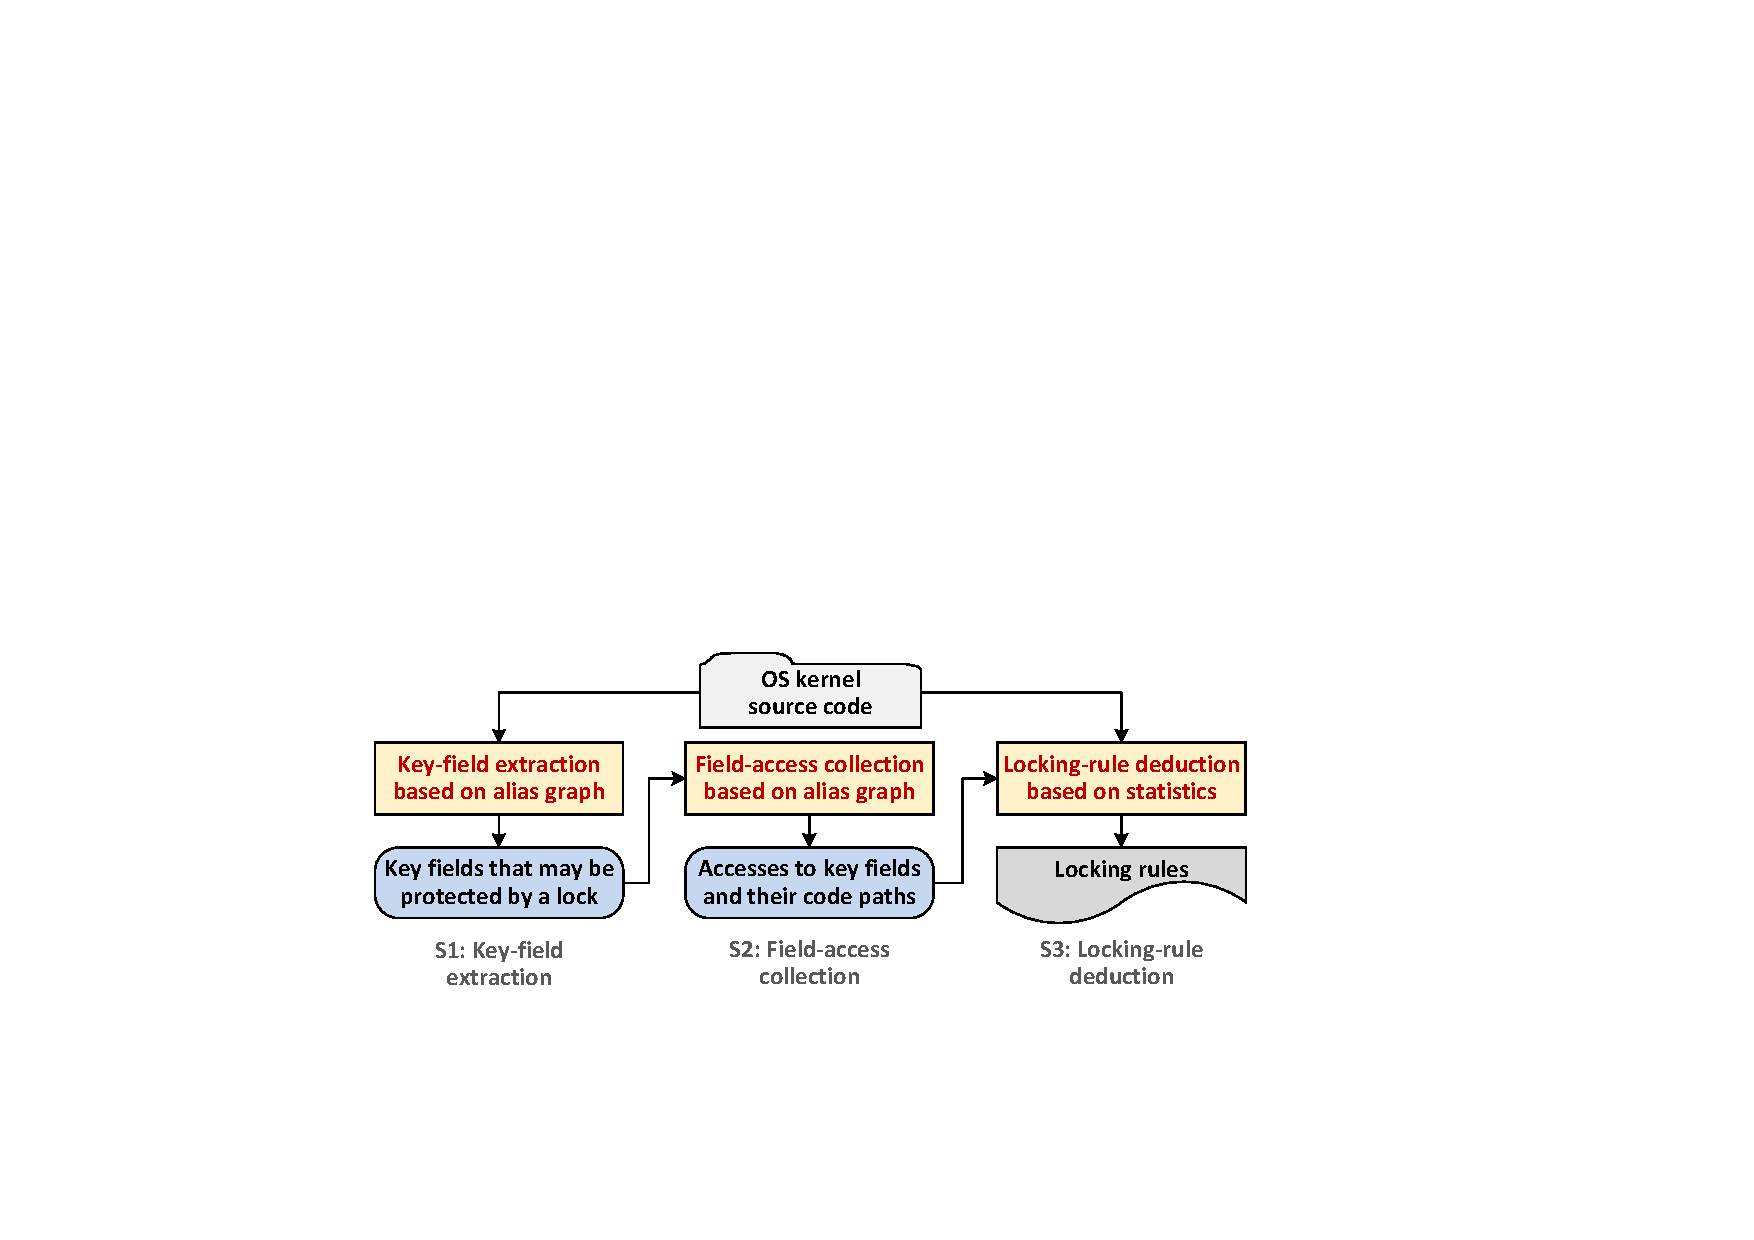
\includegraphics[width=1\linewidth]{figures/fig_workflow.pdf}
	\figcaption{Workflow of locking-rule mining.}
	\label{fig_workflow}
\end{figure}

Based on the alias graph, our alias-aware rule mining method performs an 
inter-procedural path-based~\cite{Li:ASPLOS22}, field-sensitive and alias-aware 
analysis to effectively mine locking rules about whether a specific variable 
should be protected by a lock and which lock is required. Overall, our 
alias-aware rule mining method has three main stages shown in 
Figure~\ref{fig_workflow}. In Stage 1, it extract key variable that may be 
protected by a lock. In Stage 2, it collect all accesses to key fields as well 
as code paths these accesses exist in. In Stage 3, it deduce locking rules by 
calculate the proportion of field accesses protected by a specific lock in all 
field accesses. 

\PP{S1: Key-field extraction.} The OS Kernel has a large code base with 
numerous variables. However, only a small part of variables should be protected 
by a specific lock, and thus collecting all variable accesses can introduce 
much unnecessary overhead. Generally, only a few field accesses can miss 
necessary protecting lock, due to carelessness of developers. Based on this 
insight, our analysis first extracts key fields that may need to be protected 
by a specific lock, by performing a lock-set analysis to find whether a given 
variable is accessed after acquiring a lock in the same data structure as the 
accessed field in any code path.

\begin{figure}[htbp]
	\centering
	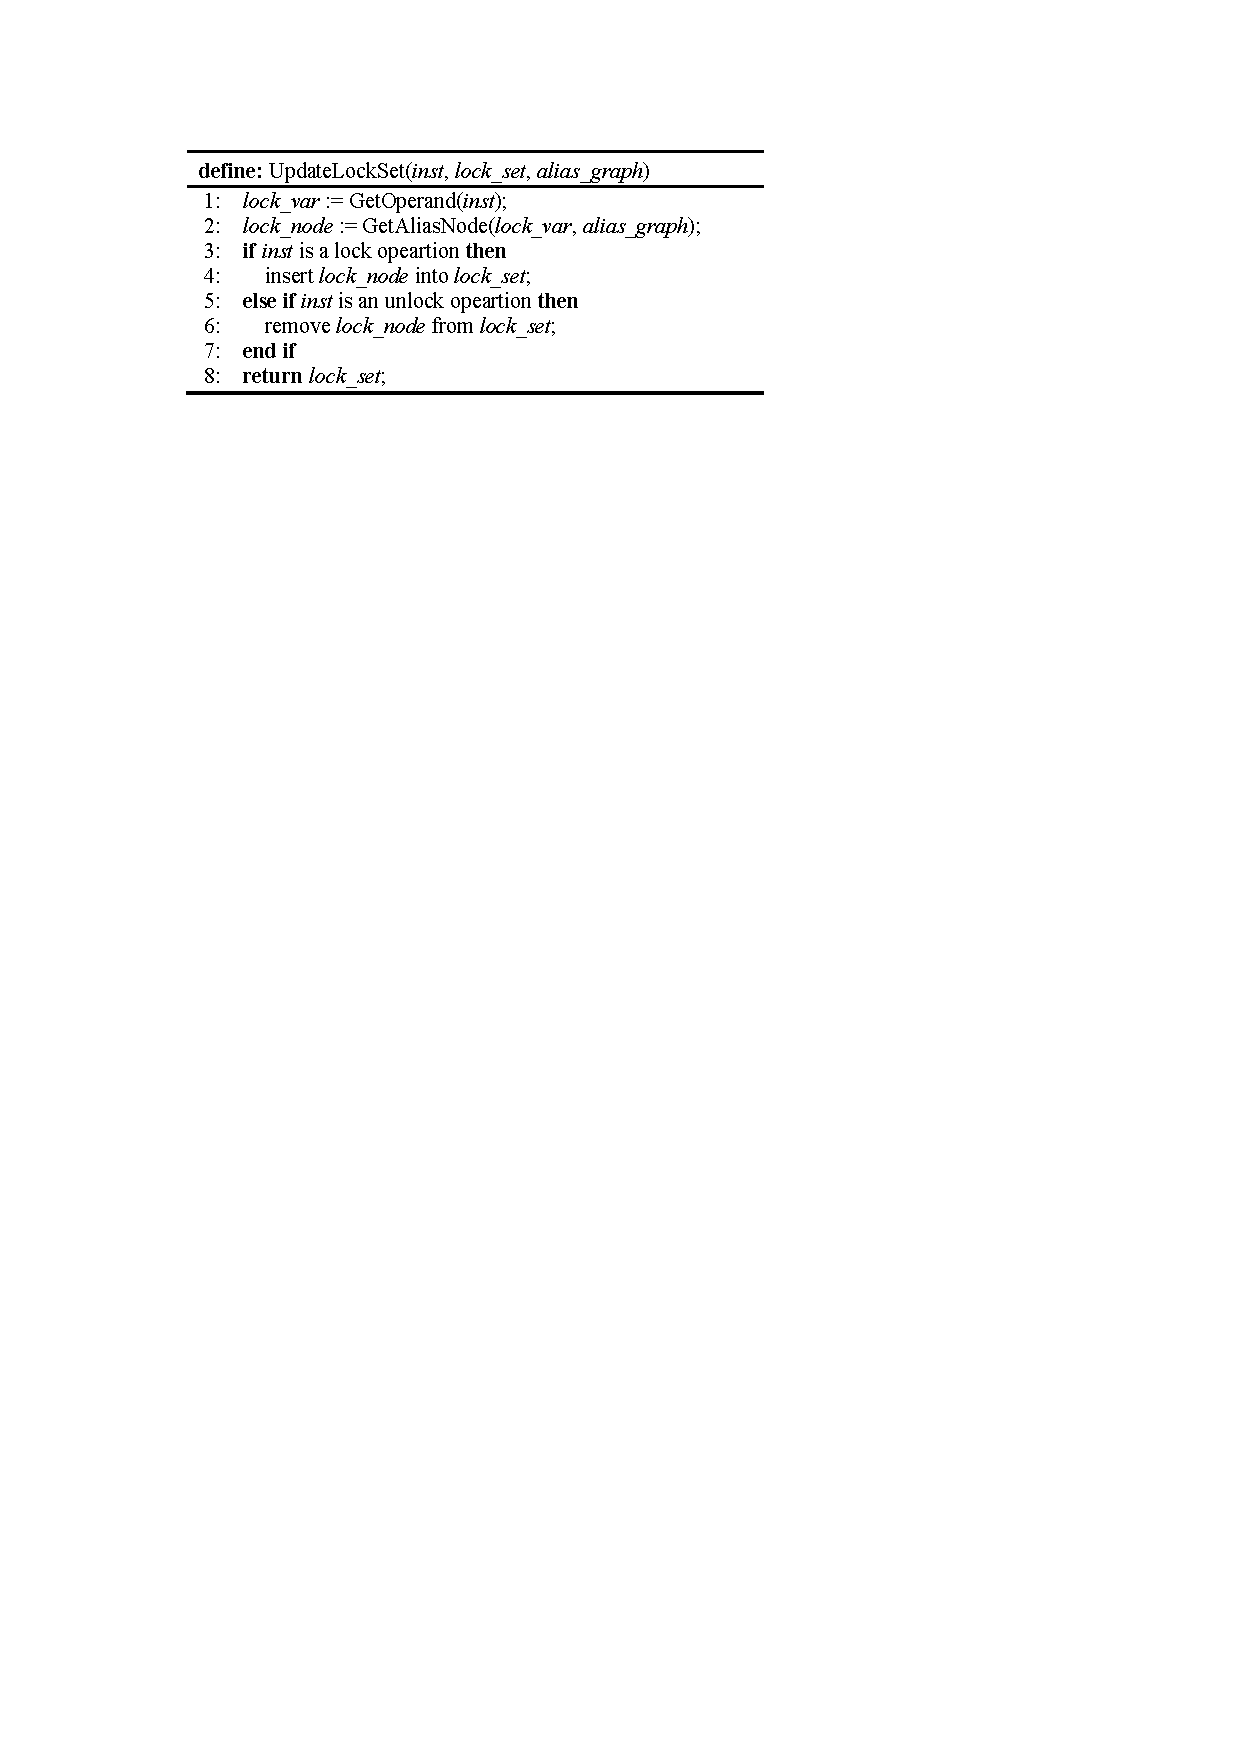
\includegraphics[width=0.9\linewidth]{figures/fig_pseudocode_lock_set.pdf}
	\figcaption{Pseudocodes of lock-set analysis.}
	\label{fig_pseudocode_lock_set}
\end{figure}

Figure~\ref{fig_pseudocode_lock_set} shows the lock-set analysis based on alias 
graph. The analysis first gets the operand of the instruction (Line 1), and 
then get the node of the operand from the alias graph (Line 2). If the 
instruction is a lock operation, the node of the operand is inserted into the 
lock set (Lines 3-4). Otherwise, if the instruction is an unlock operation, the 
node of the operand is removed from the lock set (Lines 5-6).

\begin{figure}[htbp]
	\centering
	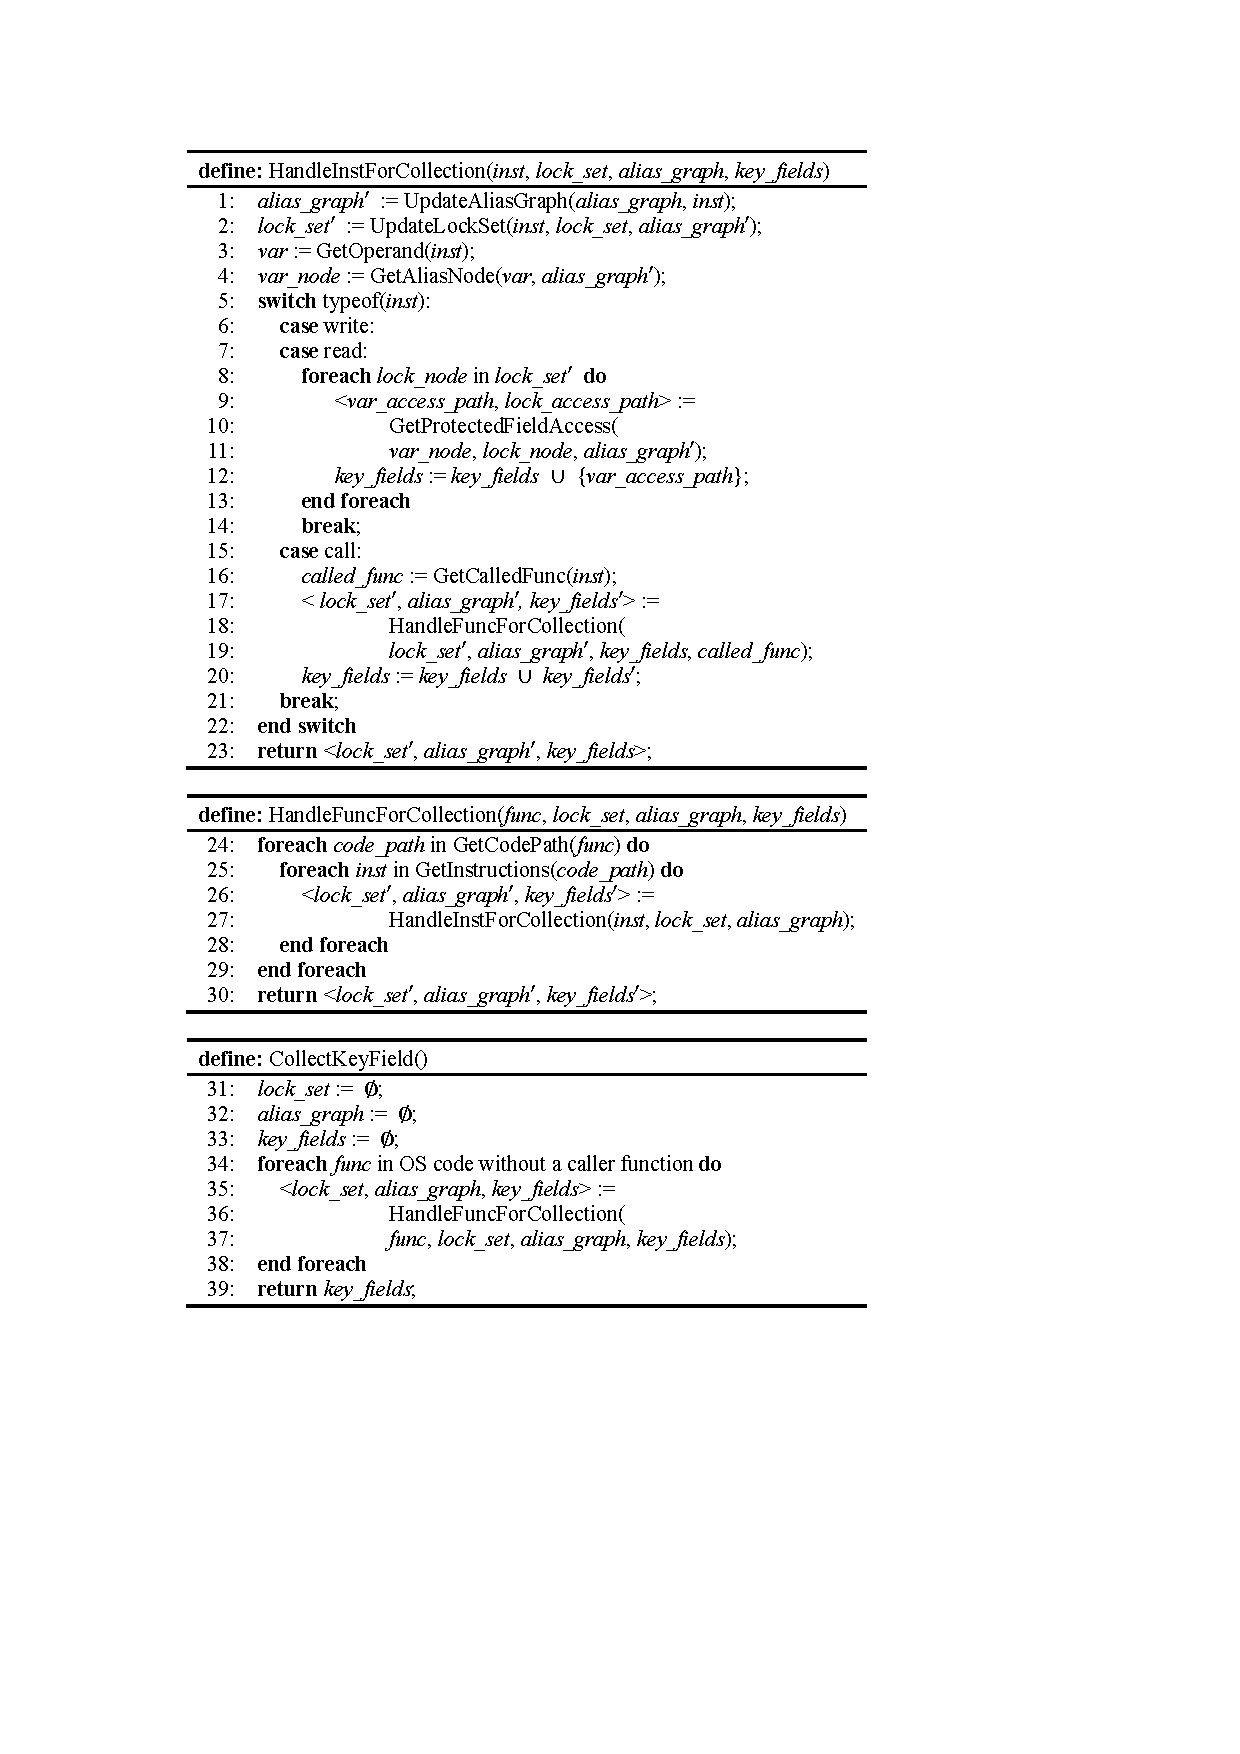
\includegraphics[width=1\linewidth]{figures/fig_pseudocode_field_extract.pdf}
	\figcaption{Pseudocodes of key-field extraction.}
	\label{fig_pseudocode_field_extract}
\end{figure}

Figure~\ref{fig_pseudocode_field_extract} shows the pseudocode to extract key 
fields that may be protected by a specific lock, based on lock-set analysis and 
the alias graph. The analysis starts from each function without a caller 
function (Lines 16-26) and performs a path-based analysis~\cite{Li:ASPLOS22} 
(Lines 17-25). For each instruction in the code path, the analysis first update 
the alias graph according to the instruction with the four operations (MOVE, 
STORE, LOAD and GEP) (Line 1), and then performs a lock-set analysis (Line 2) 
to get all acquired locks. After updating the alias graph and the lock set, if 
the instruction is a write or a read, the analysis first gets the node of the 
operand with the new alias graph (Lines 4-5). And then, for each node of 
lock variable in the lock set, the analysis uses the alias graph to extract the 
protected data structure field (Lines 6-12). If the field is not NULL, it is 
inserted into the set of key fields (Lines 9-11). For inter-procedural 
analysis, the analysis copies function definition into its call sites and this 
operation is not shown in Figure~\ref{fig_pseudocode_field_extract} for 
convenience. 

\PP{S2: Field-access collection.} With the key fields extracted in Stage 1, the 
analysis can only collects accesses to the variables that is protected in some 
cases, because if a variable is never protected by any lock when is accessed, 
it is less likely to be shared by different threads, and thus can not introduce 
no concurrency issue.

\begin{figure}[htbp]
	\centering
	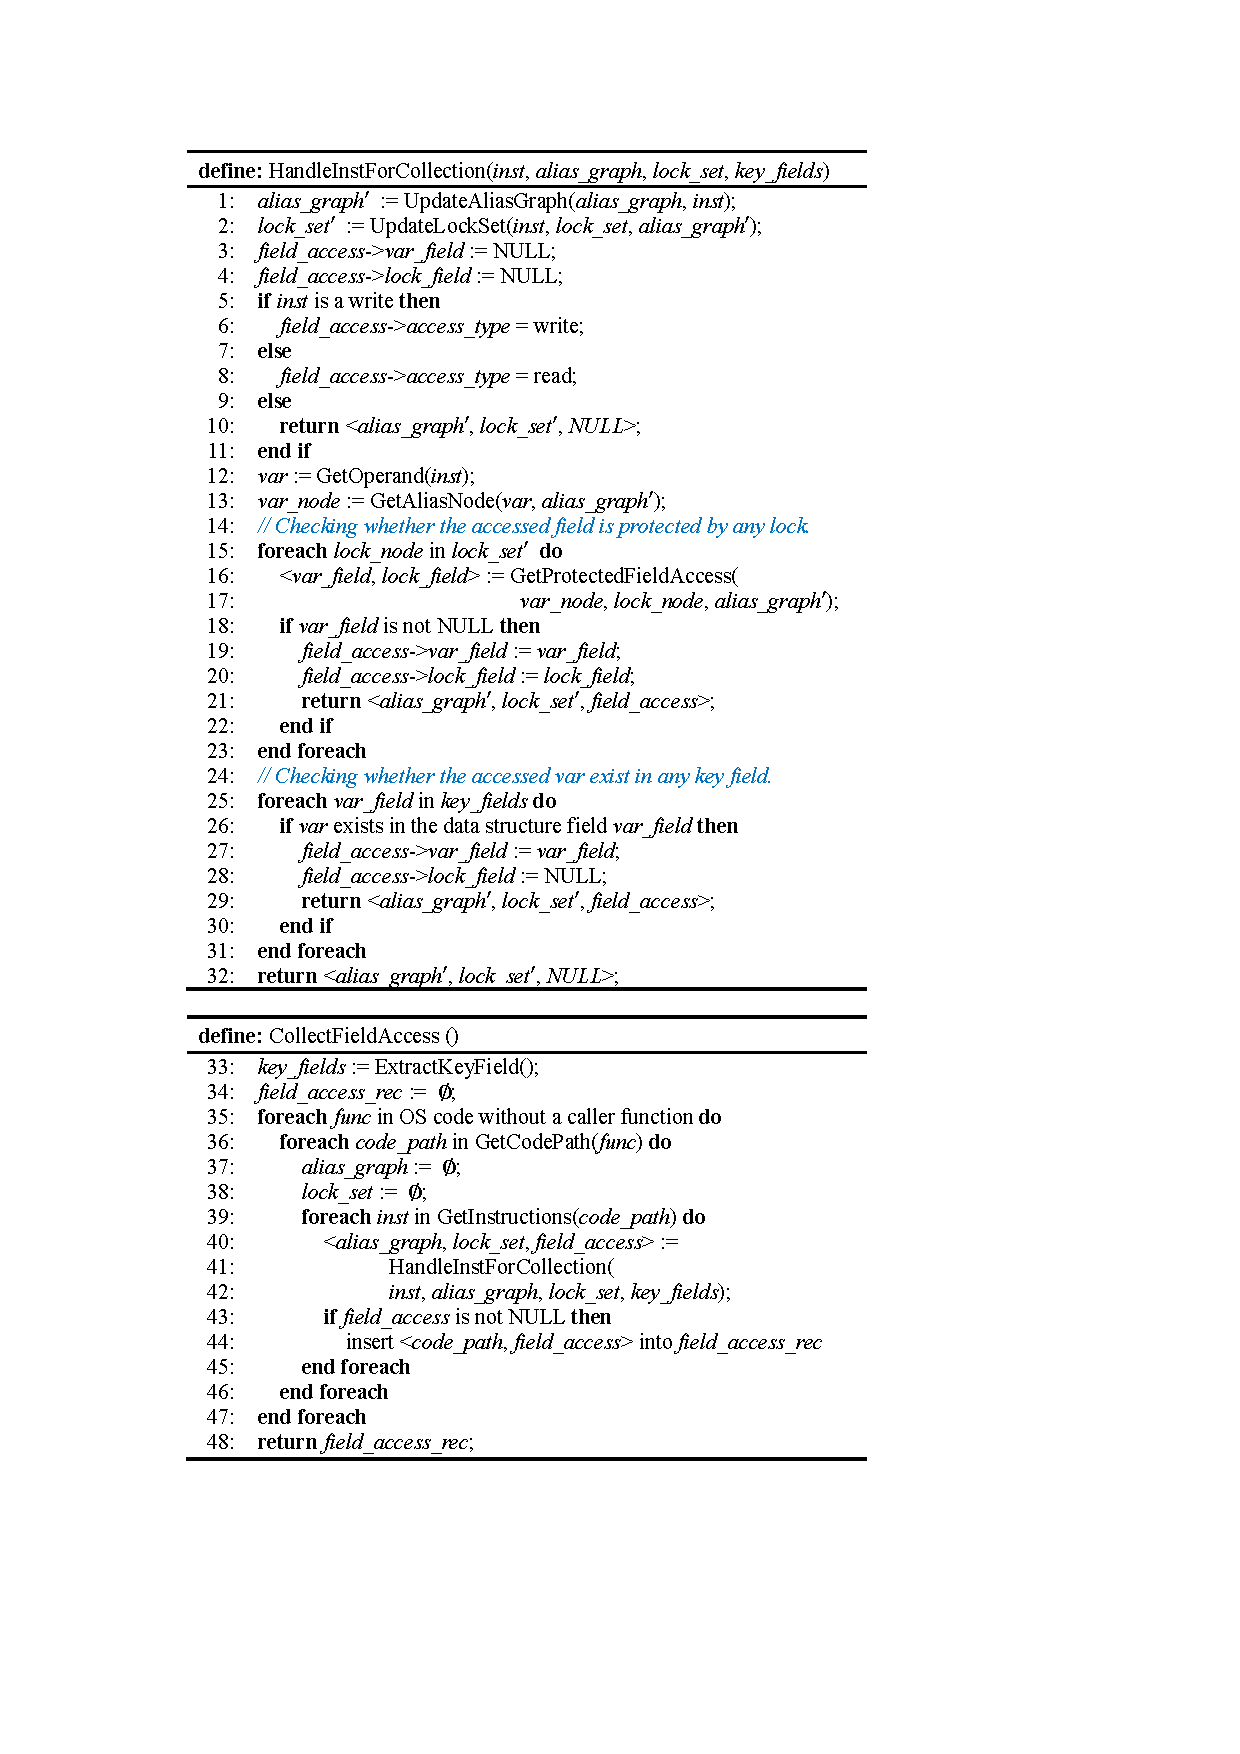
\includegraphics[width=1\linewidth]{figures/fig_pseudocode_access_collect.pdf}
	\figcaption{Pseudocodes of key-field extraction.}
	\label{fig_pseudocode_access_collect}
\end{figure}

Figure~\ref{fig_pseudocode_access_collect} shows the pseudocode to collect all 
accesses to key fields. Similarly to the key-field extraction, this stage also 
performs a path-based analysis. For each instruction in the code path (Lines 
39-45), the analysis first updates the alias graph and the lock set according 
to the handled instruction (Lines 1-2). And then, the access type (either a 
write or a read) is set according to the instruction (Lines 5-8). However, if 
the instruction is not an access operation, the function returns with a NULL 
value for the field access (Line 10). Otherwise, the analysis first gets the 
node of the operand with the new alias graph (Lines 12-13), and then for each 
node of the lock variable in the lock set, the analysis uses the alias graph 
toextract the fields that the accessed variable and the lock variable stored in 
(Lines 16-17). If the fields are found, the field access is returned with the 
found fields (Lines 18-22). If the fields are not found, the accessed variable  
does not protected by any lock. In this case, if the accessed variable is 
stored in a key field, the field access is returned with a NULL lock variable 
(Lines 25-30).

\PP{S3: Locking-rule deduction.} After collecting all accesses to key fields, 
the analysis deduces locking rules based on statistics. However, on the one 
hand, distinguishing different accesses to the same data structure field by 
different program sites is not fine-grained enough, because the access to a 
variable and the acquirement to a specific lock are often packaged in a special 
function, and all accesses under different calling context are regarded as the 
same access. On the other hand, distinguishing different accesses by different 
code paths can also suffer from inaccuracy when a function contains many branch 
statement and cause numerous code paths for the same variable access. Based on 
these consideration, the analysis distinguishes different accesses to the same 
data structure field by different calling contexts. Specifically, given a key 
field {\em f} and a lock {\em l}, the analysis first finds all access to {\em 
f} with lock {\em l} from the collected field accesses in Stage 2, and gets the 
number {\em locked\_access\_num} by counting different calling contexts 
extracted from the code paths of these field accesses. Then, the analysis finds 
all access to {\em f} (no matter which lock is accessed), and gets the number 
{\em all\_access\_num} in the same way as {\em locked\_access\_num}. If the 
ratio {\em locked\_access\_num}/{\em all\_access\_num} is larger than a given 
threshold, and these is at least one write access to {\em f}, the data 
structure field {\em f} is inferred to be protected by the lock {\em l}.

\begin{figure}[htbp]
	\centering
	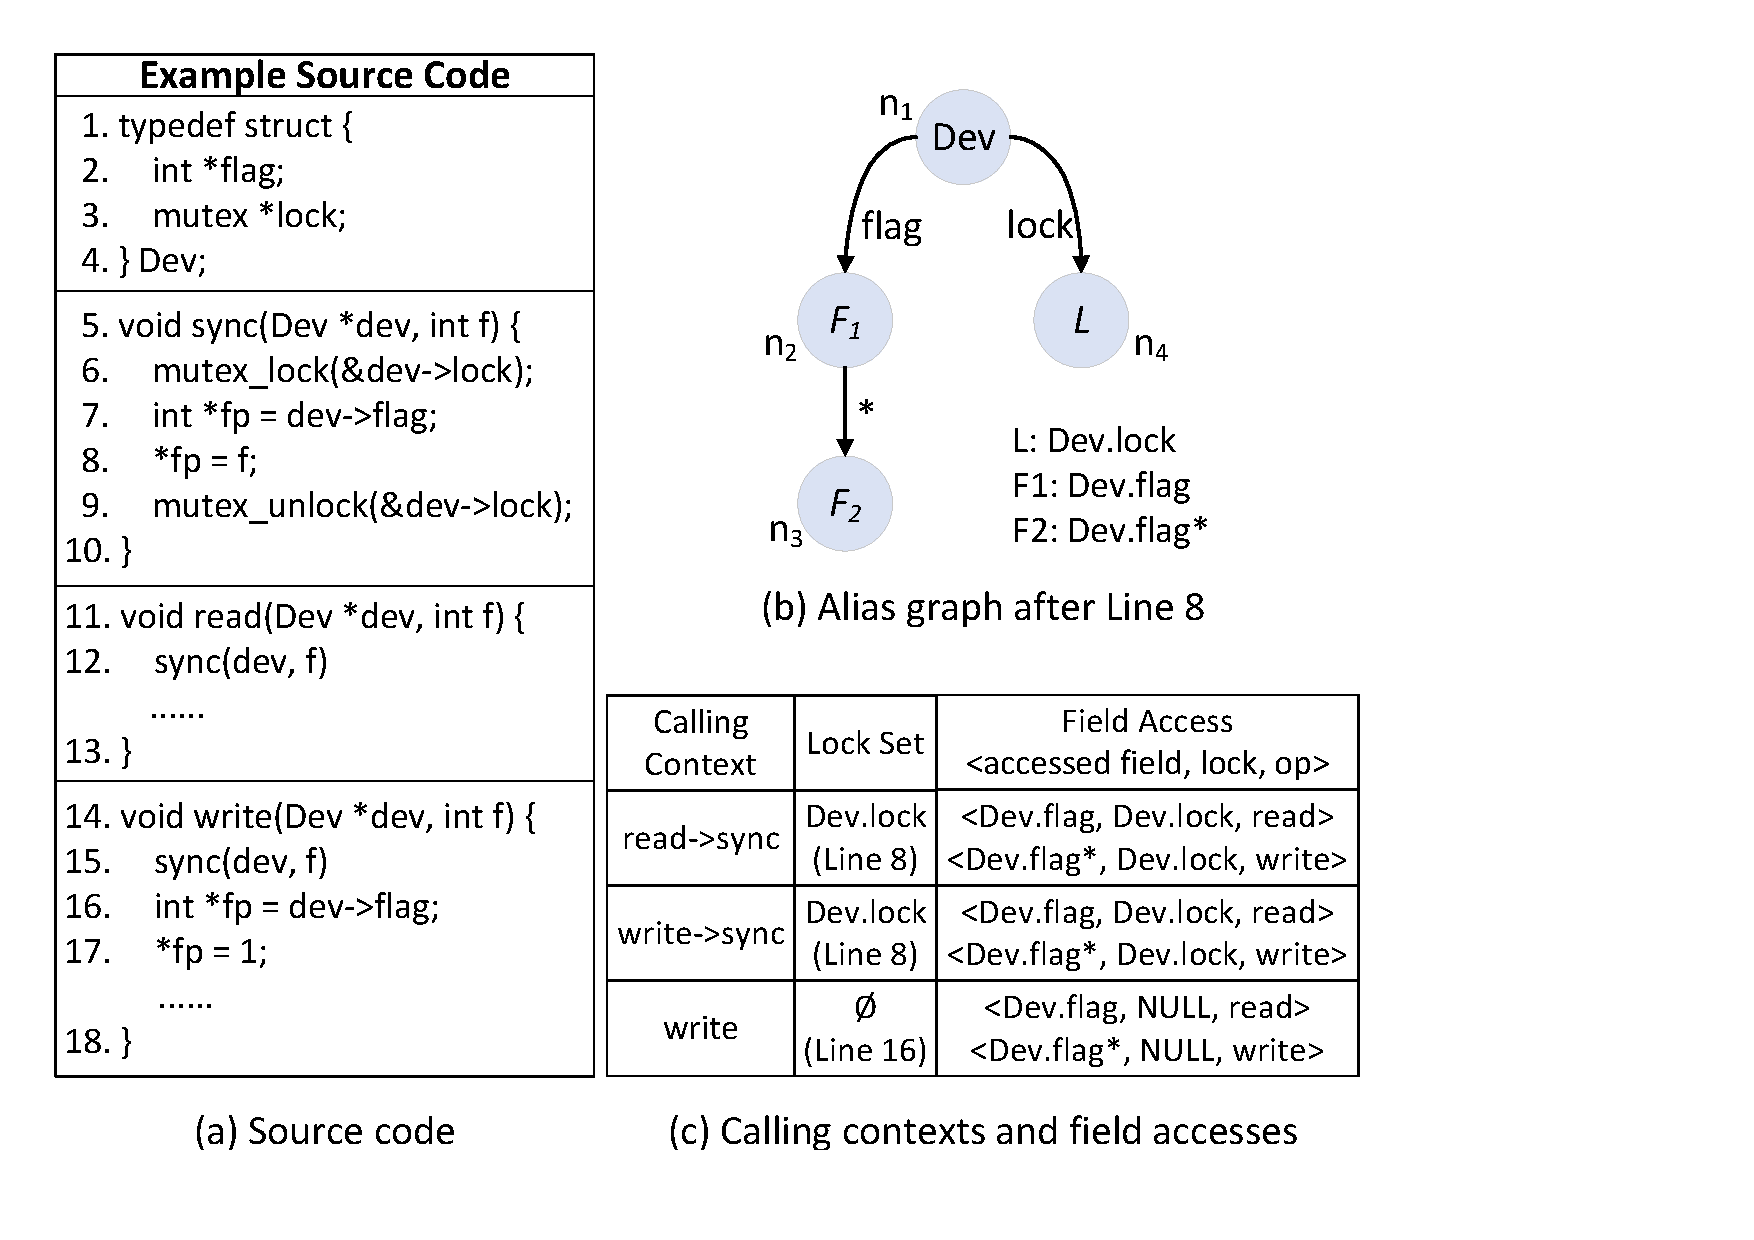
\includegraphics[width=1\linewidth]{figures/fig_demo_rule_mining.pdf}
	\figcaption{Example of locking-rule mining.}
	\label{fig_demo_rule_mining}
\end{figure}

\noindent{\textbf{\em Example.}} We use an example in 
Figure~\ref{fig_demo_rule_mining} to illustrate how to mine locking rules 
with the three stages. The analysis first perform a path-based analysis to 
extract key fields. Take the code path {\tt Line 12, Line 6, Line 7, Line 8, 
Line 9} as an example. The analysis updates the alias graph by handling two GEP 
operations ({\em \&dev->lock} and {\em fp = dev->flag}) and a STORE operation 
({\em *fp = f}). The final alias graph is shown in 
Figure~\ref{fig_demo_rule_mining}(b). At the same time of alias analysis, the 
analysis records the acquired lock {\em Dev.lock} into the lock set after the 
lock instruction at Line 6. When analyzing the read instruction at Line 7, the 
analysis finds the node of the accessed field ($\mathit{n_2}$) and the node of 
the lock stored in the lock set ($\mathit{n_4}$) has the same ancestor 
($\mathit{n_1}$), and thus {\em Dev.flag} is a key field. Similarly, {\em 
Dev.flag*} is also a key field, due to the write instruction at Line 8. 

After extracting key fields, the method collects all accesses to key fields 
with lock set analysis and the alias graph. Take the code path {\tt Line 15, 
Line 6, Line 7, Line 8, Line 9, Line 16 and Line 17} as an example, through a 
lock instruction at Line 6, the analysis records the acquired lock {\em 
Dev.lock} into the lock set. When analyzing the read instruction at Line 7, the 
analysis finds the node of the accessed field ($\mathit{n_2}$) and the node of 
the lock stored in the lock set ($\mathit{n_4}$) has the same ancestor 
($\mathit{n_1}$), and thus records a field access <{\em Dev.flag}, {\em 
Dev.lock}>. Similar to the read instruction at Line 7, the method also records 
a field access <{\em Dev.flag*}, {\em Dev.lock}> for the write instruction at 
Line 8. Then through an unlock operation at Line 9, the analysis removes the 
lock {\em Dev.lock} is removed from the lock set. As a result, the key fields 
{\em Dev.flag} and {\em Dev.flag*} are accessed without acquiring any lock, and 
thus the analysis records two field accesses <{\em Dev.flag}, {\em NULL}> and 
<{\em Dev.flag*}, {\em NULL}>. The final field accesses are shown in 
Figure~\ref{fig_demo_rule_mining}.

After collecting all field accesses, the analysis finds that the fields {\em 
Dev.flag} and {\em Dev.flag*} are accessed under three calling contexts, and 
two of them are protected by the lock {\em Dev.lock}. And thus the two fields 
{\em Dev.flag} and {\em Dev.flag*} is deduce to be protected by the lock {\em 
Dev.lock} (assume the threshold of the ratio locked\_access\_num / 
all\_access\_num is 0.6).

\subsection{Lock-Usage Analysis}
\label{subsec_lock_usage_analysis}
